\documentclass[a4paper]{article}
\usepackage{amsmath}
\usepackage{amssymb}
\usepackage{geometry}
\usepackage{enumerate}
\usepackage{natbib}
\usepackage{float}%稳定图片位置
\usepackage{graphicx,subfig}%画图
\usepackage{caption}
\usepackage[english]{babel}
\usepackage{indentfirst}%缩进
\usepackage{enumerate}%加序号
\usepackage{multirow}%合并行
\usepackage{hyperref}
\newcommand{\reals}{{\mathbb{R}}}
\hypersetup{hypertex=true, colorlinks=true, linkcolor=black, anchorcolor=black, citecolor=black}
\title{\Large \textbf{VG441 Final Exam}\\
\author{\textbf{Pan, Chongdan ID:516370910121}\\
}
}
\begin{document}
\maketitle
\begin{center}
    \textbf{\Large{THE UM-SJTU JI HONOR CODE}}
\end{center}

\noindent\textbf{I accept the letter and spirit of the honor code:\\\\
I have neither given nor received unauthorized aid on this examination, nor have
I concealed any violations of the Honor Code by myself or others.\\\\Signature:}
\section{Problem 1}
\noindent \textbf{Task 1}
    \begin{figure}[H]
        \centering
        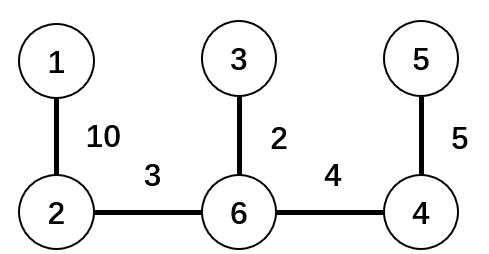
\includegraphics[scale=0.25]{P1.png}
        \caption{MST}
    \end{figure}
    \begin{figure}[H]
        \centering
        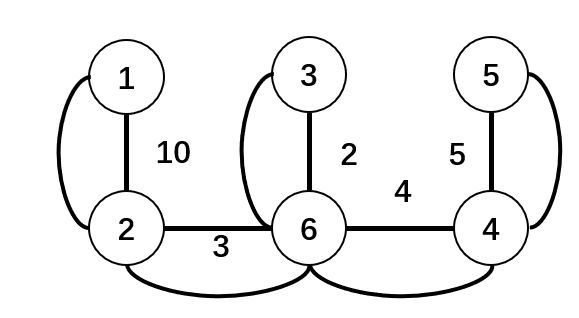
\includegraphics[scale=0.25]{P2.png}
        \caption{Double Edge MST}
    \end{figure}
    \begin{figure}[H]
        \centering
        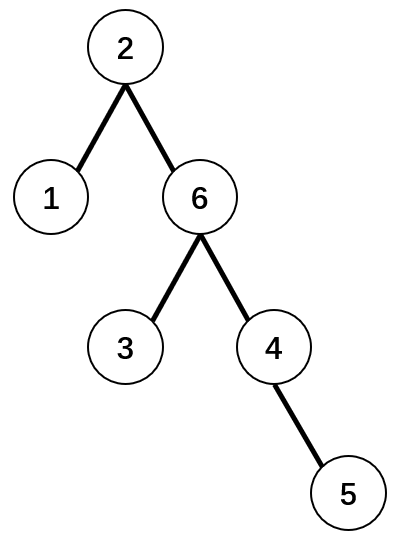
\includegraphics[scale=0.25]{P3.png}
        \caption{Eulerian Path}
    \end{figure}
    Before short cutting, our path is $2\rightarrow6\rightarrow4\rightarrow5\rightarrow4\rightarrow6\rightarrow3\rightarrow6\rightarrow2\rightarrow1\rightarrow2$
    \\After short cutting our path is $2\rightarrow6\rightarrow4\rightarrow5\rightarrow3\rightarrow1\rightarrow2$ with cost $3+4+5+86+100+10$
\\\\ \textbf{Task 2}
\\The odd degree set is $\{1,3,6,5\}$
\begin{figure}[H]
    \centering
    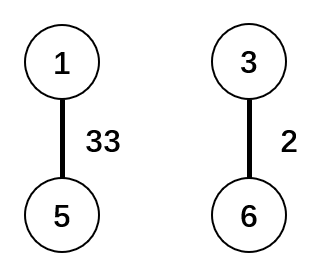
\includegraphics[scale=0.25]{P4.png}
    \caption{Min-weight-matching K}
\end{figure}
\begin{figure}[H]
    \centering
    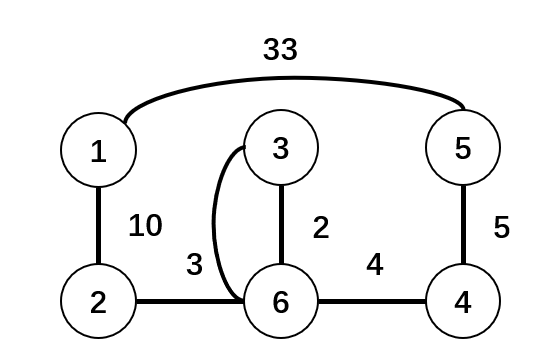
\includegraphics[scale=0.25]{P5.png}
    \caption{Add K to M}
\end{figure}
Before short cutting, our path is $1\rightarrow2\rightarrow6\rightarrow3\rightarrow6\rightarrow4\rightarrow5\rightarrow1$
\\After short cutting, our path is
$1\rightarrow2\rightarrow6\rightarrow3\rightarrow4\rightarrow5\rightarrow1$ with cost=10+3+2+6+5+33=59
\\From eyeballing solution, it's same as $1\rightarrow2\rightarrow6\rightarrow3\rightarrow4\rightarrow5\rightarrow1$ with cost=59
\section{Problem 2}
\noindent \textbf{Task 1}\\
$n=4,v_{max}=v_3=6$
\\$T[1,0]=0,T[1,4]=3$
\\$T[2,0]=0,T[2,4]=3,T[2,8]=6$
\\$T[3,0]=0,T[3,4]=3,T[3,6]=8,T[3,8]=6,T[3,10]=11,T[3,14]=14$
\\$T[4,0]=0,T[4,4]=3,T[4,5]=5,T[4,6]=8,T[4,8]=6,T[4,9]=8,T[4,10]=11$
\\$T[4,11]=13,T[4,13]=11,T[4,14]=14,T[4,15]=16,T[4,19]=19$
\\Since $T[4,9]=8$, the maximum value we can put is 9
\\\\ \textbf{Task 2}
\\After ranking, we get $\frac{v_1}{s_1}=\frac{v_2}{s_2}>\frac{v_4}{s_4}>\frac{v_3}{s_3}$
\\So we put $i_1$ and $i_2$ in the bag and the total value is 8 by occupying 6 of 8 big size, which is smaller than 9
\section{Problem 3}
\noindent\textbf{Task 1}
At first $\frac{C_1}{|S_1|}=1.2,\frac{C_2}{|S_2|}=3,\frac{C_3}{|S_3|}=1$
\\So we prefer to use $S_3$, and the remaining elements are $\{e_1,e_2,e_3,e_6,e_7\}$
\\Then $\frac{C_1}{3}=2,\frac{C_2}{|S_2|}=3$
\\So we prefer to use $S_1$ and the remaining elements are $\{e_6,e_7\}$
\\At last, we have to choose $S_3$ to cover the remaining elements.
\\In total, the cost is 6+7+15=28
\\\\ \textbf{Task 2}
\\The greedy algorithm is not optimal, since we can cover all elements with $S_2\text{ and }S_3$ and total cost is 7+15=22
\section{Bonus Problem}
\noindent \textbf{Task 1}
\\Through Lagrangian Relaxation:
$$\max_{\alpha_j,\beta_{ij}}\sum_{j\in D}\alpha_j$$
$$\text{s.t. }\sum_{j\in D}\beta_{ij}\leq f_i,\forall i\in F$$
$$\alpha_j-\beta_{ij}\leq d_{ij},\forall i\in F,j\in D$$
$$\alpha_j\geq0,\forall j\in D$$
$$\beta_{ij}\geq0,\forall i\in F,j\in D$$
\\ \textbf{Task 2}
\par Obviously, $\alpha_j$ and $\beta_{ij}$ can't be less than 0, since the demand won't contribute a negative cost. For the object, we want to maximize the amount of money demand $j$ will to contribute, when it's max, it's same to we spend least cost, since it's covered by demand.
\par The sum of $\beta_{ij}$ smaller than $f_i$ means the amount of money contributed from demands towards a facility should be less than the cost of the corresponding facilities.
\par $\alpha_j-\beta_{ij}$ represents the remaining cost after paying for the facilities, which should contribute for the demand $d_{ij}$, so it's should be smaller than $d_{ij}$ 
\end{document}